%%
%% 研究報告用スイッチ
%% [techrep]
%%
%% 欧文表記無しのスイッチ(etitle,eabstractは任意)
%% [noauthor]
%%

%\documentclass[submit,techrep]{ipsj}
\documentclass[submit,techrep,noauthor]{ipsj}


%なんかエラー出てる
%\usepackage[dvips]{graphicx}
\usepackage{latexsym}

\usepackage{cite}
\usepackage{amsmath,amssymb,amsfonts}
\usepackage{algorithmic}
\usepackage[dvipdfmx]{graphicx}
\usepackage{textcomp}
\usepackage{xcolor}
\usepackage{listings}
\usepackage{url}
\def\BibTeX{{\rm B\kern-.05em{\sc i\kern-.025em b}\kern-.08em
    T\kern-.1667em\lower.7ex\hbox{E}\kern-.125emX}}

\newcommand{\todo}[1]{\colorbox{yellow}{{\bf TODO}:}{\color{red} {\textbf{[#1]}}}}

\lstset{
basicstyle=\small\ttfamily,
abovecaptionskip=0pt,
captionpos=b,
frame=tb,
framexleftmargin=2em,
numbers=left,
numberstyle={\scriptsize},
xleftmargin=\parindent
}

%ListingのキャプションがFigureになってしまうのをListingに直すコマンド
\usepackage{caption}
\makeatletter
\let\MYcaption\@makecaption
\makeatother
\usepackage{caption}
\makeatletter
\let\@makecaption\MYcaption
\makeatother

\def\Underline{\setbox0\hbox\bgroup\let\\\endUnderline}
\def\endUnderline{\vphantom{y}\egroup\smash{\underline{\box0}}\\}
\def\|{\verb|}
%

%\setcounter{巻数}{59}%vol59=2018
%\setcounter{号数}{10}
%\setcounter{page}{1}


\begin{document}


\title{マイクロベンチマーク共有サービスを用いた\\
実行高速化のための自動リファクタリングへの試み}

%\etitle{How to Prepare Your Paper for IPSJ SIG Technical Report \\ (version 2018/10/29)}

\affiliate{WU}{和歌山大学\\
Wakayama University}

\affiliate{NAIST}{奈良先端科学技術大学院大学\\
Nara Institute of Science and Technology}

%\paffiliate{JU}{情報処理大学\\
%Johoshori Uniersity}

\author{大森 楓己}{Omori Fuki}{WU}%[s246328@wakayama-u.ac.jp]
\author{伊原 彰紀}{Ihara Akinori}{WU}
\author{柏 祐太郎}{Kashiwa Yutaro}{NAIST}

\begin{abstract}
プログラムには同じ結果が得られる複数の実装方法が存在し,それぞれで実行速度が異なる.実装経験豊富な開発者であっても高速なプログラム実装方法の検討は困難を極める.本研究では,ソフトウェアの部分的なプログラムの実行速度を計測するためのマイクロベンチマークと呼ばれる検証サービスで公開されたデータセットを用いて,既存の大規模言語モデルに学習させ,実行速度の改善に特化した自動リファクタリングモデルを構築し,性能を評価する.
\end{abstract}


%
%\begin{jkeyword}
%情報処理学会論文誌ジャーナル,\LaTeX,スタイルファイル,べからず集
%\end{jkeyword}
%
%\begin{eabstract}
%This document is a guide to prepare a draft for submitting to IPSJ
%Journal, and the final camera-ready manuscript of a paper to appear in
%IPSJ Journal, using {\LaTeX} and special style files.  Since this
%document itself is produced with the style files, it will help you to
%refer its source file which is distributed with the style files.
%\end{eabstract}
%
%\begin{ekeyword}
%IPSJ Journal, \LaTeX, style files, ``Dos and Dont's'' list
%\end{ekeyword}

\maketitle

%1
\section{はじめに}
プログラムは,外的振る舞いの等しい別のプログラムに書き換えることでその品質を向上できることがある.そのような改良はリファクタリングと呼ばれ,保守性や性能効率性等のさまざまな品質を高めるために行われる.例として,Webアプリケーション開発ではリファクタリングを行うことでプログラムの実行時間を25\%から70\%高速化している\cite{Selakovic_2016}.

リファクタリングはプログラム開発における重要なステップであり,%\todo{もっとリファクタリングは難しいとかの話の方が,なんで自動化する必要があるかがわかりやすい}
その効率化のため%欠陥箇所の検出\todo{関係ある?最低でも参考文献}や修正を自動化する
の手法が多数提案されている.例として,プログラムの可読性は命名規則違反や文法上の欠陥を検出する静的解析ツール%\todo{上で効率化の話をだしているんだから,また抽象的な話に戻さない方が良い.ルールベースの方法とかが提案されているとかない?Selakovicらの正規表現とか}
\footnote{\url{https://eslint.org/}}\footnote{\url{https://biomejs.dev/}}を用いて維持・向上でき,さらに
%によって欠陥箇所を容易に特定することができ,
検出された問題の多くは自動的に修正できる\footnote{\url{https://biomejs.dev/linter/rules/}}\footnote{\url{https://eslint.org/docs/latest/use/command-line-interface#fix-problems}}.%\todo{引用}
一方で,%実行速度の遅いプログラムに対する自動修正に関する研究は著者らの知る限り数少ない.\todo{ここで一つぐらい従来研究を入れられるといいけど.}
プログラムの実行速度に対しては,ベンチマークテストを用いた定期的な実行速度の測定による速度低下の早期発見,および原因箇所の特定手法が存在するものの,実行を速めるための改良には,%静的解析ツールには登録されていない,
糖衣構文や外部ライブラリ等を用いた
%\todo{「依存した非自明な」$\leftarrow$いるかな?}
広範な代替実装
%を発見するため
の知識を要する.さらに,JavaScriptに代表される動的型付け言語は,単一の変数に異なる型のオブジェクトを再代入できるため,
%静的解析によるトレースが困難である\todo{引用}ため,
代替可能な実装箇所の発見には文脈に基づく高度な技術的判断を要する.これは多くの動的型付け言語がインタプリタ言語であり,その実行速度がコンパイラ言語に比べて遅いことを考えると,非常に重要な課題である.%\todo{誰にとっての問題かな?課題で良いのでは?}

%\todo{ここ以降は,1章にしては長すぎる.この前で,手法を提案する.JsParfを活用する.とかで良いかと.今書いているのは2章に持っていく.タイトルを背景にするなど}
%では,実行速度の欠陥を修正する開発者はどのように代替実装の知識をどのように学習することができるか? 
実行速度を改善するための代替実装の知識を習得し,他の実装者と共有するために,JavaScriptではマイクロベンチマーク共有サービスとしてJsPerf\footnote{JsPerf: \url{https://jsperf.app/}}やMeasureThat.net\footnote{MeasureThat.net: \url{https://measurethat.net/}}がある.これらのサービスを介して,開発者はJavaScriptプログラムをブラウザ上で実行し,その実行速度を測定できる.開発者は外的振る舞いが互いに等しいJavaScriptプログラム同士の実行速度を比較することで,より高速な実装を確認できる.さらに,比較されたプログラムセットは保存され,すべてのユーザに公開される.このプログラムセット(大抵は非常に短いコードスニペット)はマイクロベンチマークと呼ばれる.開発者は,サービスに保存されているマイクロベンチマークを検索することで未知の実装を学習できる.Listing~\ref{setup}およびListing~\ref{test-a},Listing~\ref{test-b}にマイクロベンチマークの例を示す.%\todo{listing1,2,3を1つにまとめたい.}

%----------------------------------
\begin{figure*}[t]
\captionsetup{name=Listing}
  \caption{Setup}\label{setup}
\begin{lstlisting}
var i, array = []
for(i=0; i<10000; i++)
    array[i] = i;
\end{lstlisting}
  \begin{minipage}[b]{0.48\linewidth}
  \caption{Test Program 1}\label{test-a}
\begin{lstlisting}[firstnumber=4]
for(i=0; i<array.length; i++)
    console.log(array[i]);
\end{lstlisting}
  \end{minipage}
    \hspace{0.07\columnwidth} % ここで隙間作成
  \begin{minipage}[b]{0.48\linewidth}
    \caption{Test Program 2}\label{test-b}
\begin{lstlisting}[firstnumber=4]
array.forEach((item) => console.log(item));
\end{lstlisting}
  \vspace{3.5mm}
  \end{minipage}
\end{figure*}
%----------------------------------

マイクロベンチマーク全体は,1つのセットアッププログラムと1つ以上のテストプログラムから構成され,各テストプログラムを実行する前にセットアッププログラムが実行される.マイクロベンチマーク共有サービス上では,セットアッププログラムの実行速度は測定されず,テストプログラムの実行速度のみが測定される.次に両プログラムの役割について述べる.



\begin{description}

\item[セットアッププログラム(Listing~\ref{setup}を参照)]\mbox{}\\
実行速度を測定する前に,テストプログラム中で用いる配列や関数を定義するプログラム部である.1つのセットアッププログラムが,すべてのテストプログラムに共通して用いられる.例として,Listing~\ref{setup}では後にテストプログラム(Listing~\ref{test-a}および\ref{test-b})で使用する配列を定義している.

\item[テストプログラム(Listing~\ref{test-a},\ref{test-b}を参照)]\mbox{}\\
実行速度を測定する1つ以上の実装を記述するプログラム部である.例としてListing~\ref{test-a}および\ref{test-b}では,外的振る舞いが互いに等しい2つの実装をそれぞれ記述している.

\end{description}


これらのサービスは膨大かつ多様なマイクロベンチマークを提供するが,これを用いた実行速度の自動改善手法は著者らの知る限り提案されていない.本研究では,マイクロベンチマーク共有サービスからリファクタリングのための大規模なデータセットを作成し,実行速度の向上のためのLLMベース自動リファクタリングモデルを作成する.さらに既存の対話型人工知能と比較することで,%マイクロベンチマーク共有サービスのプログラムの学習によって自動修正できるプログラムを明らかにする.\todo{精度評価しかしていない場合,明らかになっていないことになるので要注意.}
マイクロベンチマーク共有サービス上のプログラムを学習した大規模言語モデルの修正性能を明らかにする.

続く\ref{sec:related}章では,本研究の関連研究について述べる.\ref{sec:method}章では,本研究の提案手法について述べ,\ref{sec:evaluation}章では評価手法について述べる.そして\ref{sec:result}章で評価結果,\ref{sec:threats}章で本研究の妥当性の脅威を述べた後,最後に\ref{sec:conc}章で総括する.

%%%%%%%%%%%%%%%%%%%%%%%%%%
%2
\section{関連研究}\label{sec:related}
%%%%%%%%%%%%%%%%%%%%%%%%%%

Selakovicら\cite{Selakovic_2016}は,JavaScriptプロジェクトにおいて開発者が高速化のために行ったリファクタリングを調査した.その結果,リファクタリングされたプログラムの半数が改良の後テストに失敗している%\todo{「改良前後で振る舞いが変わっている」ってこと?}
ことを明らかにした.この結果は本研究の動機づけとなっている.%\todo{本当はここで動機付けをもっと書きたい}
また,\cite{Selakovic_2016}はJavaScriptプロジェクトの解析によって10件の頻出する改良パターンを作成している.この改良パターンを用いた自動修正モデルは一定の高速化効果を示しているが,多様なリファクタリングを網羅するには至っていない.本研究では,マイクロベンチマークから大規模なデータセットを構築することによって,より広範なプログラムを対象とした自動リファクタリングモデルを作成する.

Gongら\cite{Gong_2015}はJITコンパイラによる高速化のアンチパターンとなるプログラムをJIT-unfriendlyと形容し,JIT-unfriendlyなプログラムに対する修正パターンを7件提案した.この修正パターンのマッチングは動的解析によって取得した情報を用いる点で,本研究の提案モデルに比べて優位性を持つ.本研究では,静的解析のみを用いた最新の大規模言語モデルに基づく自動リファクタリングの性能を明らかにする.

Selakovicら\cite{Selakovic_2017}は条件式の演算順序に着目し,動的解析と探索的手法を用いて条件演算を最適化する自動修正モデルを提案した.このモデルは探索的手法を用いる点で,局所的な実装の修正による高速化の1つの上限を示す.本研究は,探索的手法の代わりに大規模言語モデルを用い,より広範な修正機会の発見を目指す.

最後に,近年では対話型人工知能を活用したリファクタリング手法が多く提案されている
%大規模な開発履歴を活用した深層学習によるプログラム自動生成手法が多く提案されている
\cite{Ishizue_2024}\cite{Shirafuji_2023}ことも特筆する.%\todo{話が大きく変わるな〜節にするか,見出しをつけるかした方が良い気がする}
%特にOpenAIによって開発されたChatCPTモデルはソフトウェア開発のみならず,非常に広範なタスクで人間の専門家に近い性能を誇る.\todo{不要}\todo{これは6,7で使われているの?全体的に苦しいな.以下の研究でChatGPTがパフォーマンス向上に使われていることがわかっているから,それを使っても良い.・Unveiling ChatGPT's Usage in Open Source Projects: A Mining-based Study//・On the Use of ChatGPT for Code Review//・Artificial Intelligence vs. Software Engineers: An Empirical Study on Performance and Efficiency Using ChatGPT}
しかし,%その詳細な学習データセットは公開されておらず,高速化修正タスクにおける性能は明らかでない.
一般に開発者が行うリファクタリングは複数の品質を考慮することが多く,他の品質(例えば可読性)を向上させるために実行速度を低下させるような修正や,改良に失敗しているような修正も行われることがある.頻繁に行われる改良が必ずしも高速化にとって最適とは限らないため,既存の大規模言語モデルが最適な代替実装を提案するとは限らない.提案手法は高速化の観点からのみ学習データセットを作成するため,特定の領域では既存手法を上回ると考える.本研究では,最新の対話型人工知能であるChatGPT-4oと提案手法による生成プログラムを比較し,提案手法の修正性能を明らかにする.


%%%%%%%%%%%%%%%%%%%%
%3
\section{方法論}\label{sec:method}
%%%%%%%%%%%%%%%%%%%%

プログラムの実行を速める自動リファクタリングモデルを作成するため,マイクロベンチマーク共有サービス上のプログラムから互いに代替可能な実装対を作成する.そして,既存の大規模言語モデルを収集した実装対を用いてファインチューニングし,高速化のためのリファクタリングタスクを適用する.実装対の作成および自動リファクタリングモデルの作成概要を図\ref{fig-overview}に示し,以降で各手順を説明する.


\begin{figure*}[t]
\centerline{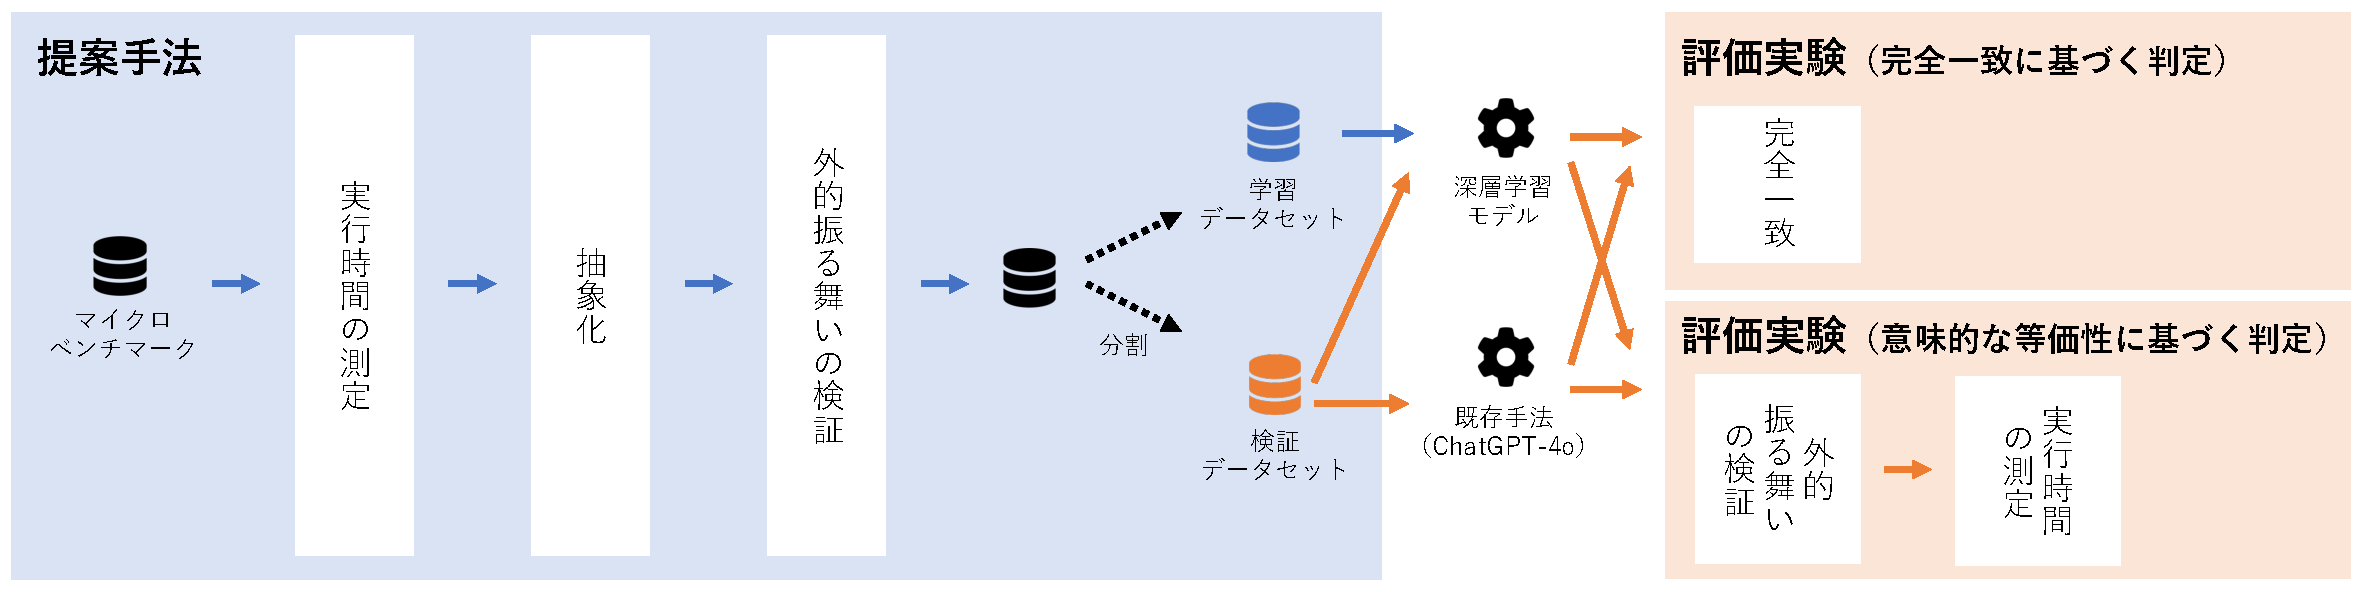
\includegraphics[width=0.9\linewidth]{Omori_fig/overview.pdf}}
\caption{overview}
\label{fig-overview}
\end{figure*}


\subsection{マイクロベンチマークの収集}
本研究では,Saikiら\cite{Saiki_2021}がマイクロベンチマーク共有サービスJsPerfから収集したプログラムセットをデータセットに用いる.ただし,JsPerfには既存のマイクロベンチマークを修正し,新たなリビジョンとして保存する機能が有るため,複数のリビジョンを持つマイクロベンチマークによってデータセットが偏るおそれがある.これを防ぐため,以降の手順では最新リビジョンのプログラムセットのみを用いる.
%\todo{できればSetupと比較プログラムを合わせてトピックのような名前をつけておきたい.}
さらに,データ整形やモデル構築に長大な時間を要するため,文字数が多い上位5\%のプログラムをデータセットから除外する.

\subsection{実行時間の測定}\label{subsec:measureTime}

JsPerfのWebサービス上にも実行速度の計測結果が保存されているが,本研究で自動生成したプログラムと比較するため,著者らの実行環境で実行時間を測定する.本研究では,マイクロベンチマーク中のセットアッププログラムとテストプログラムを結合し,プログラム全体の時間を測定する.測定後,実行時間の長いプログラムと短いプログラムを対応づけ,修正前後の対を作成する.測定手順は従来研究\cite{Selakovic_2016}に従う.まず,NVMインスタンスを起動し,\begin{math}N_{warmUp}\end{math}回プログラムを実行する.これにより,JITコンパイラをウォーミングアップさせる.続けて,\begin{math}N_{measure}\end{math}回プログラムを実行し,その実行時間を測定する.この手順を繰り返して\begin{math}N_{NVM}\end{math}回の測定を行い,プログラムごとに\begin{math}N_{NVM}\end{math}個の測定結果を得る.本研究では,テストプログラムについてプログラム1回の実行時間や計測器の分解能を考慮して\begin{math}N_{warmUp}=5\end{math},\begin{math}N_{measure}=1,000\end{math},\begin{math}N_{NVM}=10\end{math}に設定する.また,JavaScript実行環境にはNode.jsを用いる.すべての測定はCPUコア数12のIntel(R) Xeon(R) Silver 4214R CPU @ 2.40GHz上で行う.

測定結果から実行時間の95\%信頼区間を算出し,その閉区間に重なりのない実装対を作成する.以上の手順によって,68,821組の実装対を作成した.次の手順では,この実装対のうち実行時間の長い方を修正元,短い方を修正先としてその変換をモデルに学習させる.

\subsection{前処理}
従来研究で作成されるプログラム自動修正モデルでは,作成時に汎化性能を高めるため学習プログラムセット中の変数名や関数名,リテラルの抽象化を行うことが多い.本研究でも同様にプログラムセットに対して抽象化を施す.ただし,一般的なプログラム自動修正モデルがバグ修正への利用を目的として作成されるのに対して我々の提案手法はリファクタリングへの利用を目的としているため,バグ修正タスクとは異なる手法で抽象化を施す.具体的には,変数名,関数名,リテラルのうち,特定のトークンのみを抽象化する.それぞれの抽象化基準について順に説明する.

\begin{description}

\item[変数名]\mbox{}\\
プログラム中で宣言されている変数のみを抽象化する.プログラム\ref{test-a}中のlengthのようなプログラム中で明示的に宣言されていないメンバ変数は,同等の実装において常に固定の変数名を持つため,抽象化しない.抽象化後の変数名は,VAR\_1,VAR\_2,…のようにする.実装対の両方に共通する変数名は,同一の変数名に抽象化される.

\item[関数名]\mbox{}\\
変数名と同様に,プログラム中で宣言されている関数のみを抽象化する.抽象化後の関数名は,FUNCTION\_1,FUNCTION\_2,…のようになる.

\item[リテラル]\mbox{}\\
すべてのリテラルを抽象化しない.リテラルを抽象化することで修正を捉えられなくなるパターンが一定数存在するためである.例として,Listing~\ref{unmatched-literals-a}とListing~\ref{unmatched-literals-b}の実装対を示す.両プログラムはどちらも小数n=1.234から小数第2位までの概数(すなわち,1.23)を求める実装である.実装が異なるため,両プログラム内で使用する関数とその引数リテラルが異なるが,両者の引数リテラル(2と100)には暗黙的な対応関係(\begin{math}\log_{10} 100=2\end{math})がある.このような場合にリテラルを抽象化すると,深層学習モデルは暗黙的な対応関係を学習する機会を失うとともに,修正元に存在しないリテラルを含む修正候補を生成できない.これを防ぐため,リテラルはすべて抽象化しない.

\end{description}

\begin{lstlisting}[caption=Pair of unmatched literals 1, label=unmatched-literals-a,captionpos=t]
let n = 1.234;
n.toFixed(2);
\end{lstlisting}

\begin{lstlisting}[caption=Pair of unmatched literals 2, label=unmatched-literals-b,captionpos=t]
let n = 1.234;
Math.round(n*100)/100;
\end{lstlisting}


実装対の両方に共通する変数名や関数名の抽象化後トークン名を一致させるため,GumTree\cite{Falleri_2014}を用いて修正元のプログラムと修正先のプログラムの共通部分を検出した.

また,マイクロベンチマーク内でセットアッププログラムが共通して用いられるため,プログラム中に使用されていない変数や関数が有る場合がある.このようなコードスニペットは学習の妨げになるため,プログラムから除去する.使用されていない変数や関数の検出には,静的解析ツールESLintを使用する.

例としてプログラム\ref{test-a}および\ref{test-b}に対して前処理を行った場合,最終的なプログラムはListing~\ref{abstract-a},\ref{abstract-b}のようになる.


\begin{lstlisting}[caption=Abstracted Program 1, label=abstract-a,captionpos=t]
var VAR_1, VAR_2 = []
for(VAR_1=0; VAR_1<10000; VAR_1++)
    VAR_2[VAR_1] = VAR_1;

for(VAR_1=0; VAR_1<VAR_2.length; VAR_1++)
    console.log(VAR_2[VAR_1]);
\end{lstlisting}

\begin{lstlisting}[caption=Abstracted Program 2, label=abstract-b,captionpos=t]
var VAR_1, VAR_2 = []
for(VAR_1=0; VAR_1<10000; VAR_1++)
    VAR_2[VAR_1] = VAR_1;

VAR_2.forEach((VAR_3) => console.log(VAR_3));
\end{lstlisting}


\subsection{データクレンジング}\label{subsec:clean}
JsPerfで評価されたプログラム実装対を目視調査した結果,実装対の中に外的振る舞いが等価でない実装対が多く含まれることが分かった.そのため,プログラムの外的振る舞いを検証し,等価でない実装対をデータセットから除外する.検証する実装対は68,821組にも及ぶため,自動検証手法について検討した.
%最終的に独自の検証アルゴリズムを用いた.
テスト自動生成手法や対話型人工知能による検証手法が考えられるが,マイクロベンチマーク共有サービス特有の実装方法を正しく判定できない事例が存在することを確認したため,使用しないこととした.例として,Listing~\ref{unmatched-literals-a}とListing~\ref{unmatched-literals-b}のように演算結果を変数に格納することも標準出力に出力することもない事例がある.このような演算は厳密には外的振る舞いに関係しないが,意味的に等価でない実装対の学習はモデル性能の低下につながる恐れがある.これは演算結果でなく演算過程を検証するマイクロベンチマークに特有の問題である.このような実装に対して,自動生成テストでは意味的等価性を検証できない.我々はプログラム中の式を検出し,その演算結果を確認することでこの問題に対処する.

また,ArrayとUint32Arrayのようにクラスが異なるインスタンス同士でも互換性がある事例に対しても,型の一致を検証する自動生成テストでは意味的等価性を検証できない.同様に,最新の対話型人工知能も自然言語によるガイドラインを与えない場合には型の不一致を理由に意味的に等価でないと判定することを確認した.この問題に対処する最も単純な解決手法は,等価な型とみなすセーフリストを作成することであるが,膨大な実装対から意味的に等価な型を網羅することは現実的ではない.本研究ではプログラムの意味的な等価性を検証するために次のアルゴリズムを提案する.

\begin{description}

\item[標準出力の比較]\mbox{}\\
第一に,プログラム間の標準出力を比較し,一致しない実装対を除外する.実行前にDate.now()関数やMath.random()関数のような,参照等価でない代表的な関数は返却する値を固定し,参照等価になるよう設定する.

\item[終了時の変数格納値の比較]\mbox{}\\
第二に,プログラム終了時の変数格納値を比較し,一致しない実装対を除外する.変数の抽出にはプログラムの抽象構文木を作成して用いる.また,プログラム中で同名の変数を同一用途とみなし,すべての変数対の格納値が一致する場合,意味的に等価であると判定する.実装対のうち,片方のプログラムでのみ定義された変数については一致を確認せず,両方のプログラムで定義された変数についてのみ一致を確認する.また,ArrayとUint32Arrayのように型は異なるが意味的に等価である事例に対処するため,変数格納値はtoString()メソッドを用いて文字列に変換した後,一致を確認する.ArrayとUint32Arrayのように型が異なる場合でも変換後の文字列は同一であるため,これを利用する.ただし,連想配列は内部の値に関係なくすべて同一の文字列に変換されるため,別にvalueOf()メソッドを使用する.toString()メソッドもvalueOf()メソッドもObject型に実装されており,JavaScriptにおけるほぼすべてのオブジェクトはObjectのインスタンスであるため,これらのメソッドは多くの変数格納値に対して呼び出せる.ただし,例外的にObjectではない値(null)やプログラム終了時点でグローバルスコープに無い変数に対してメソッドの呼び出しを行い,値を取得できなかった変数対に対しては一致を確認せず,それ以外の変数についてのみ一致を確認する.

\item[式のみの場合の比較]\mbox{}\\
目視調査の結果,結果を変数に格納することも標準出力に出力することもない演算の多くは1行のみのテストプログラムに多いことが分かった.そのため,実装対の両方のテストプログラムが1行(すなわち,最後の1文以外の全文が同一)で,最後の文が式としても評価できる場合には,その演算結果を比較し,一致しない実装対を除外する.

\end{description}

最終的に29,809組の外的振る舞いが等しい実装対を抽出した.

\subsection{モデル構築}
\subsubsection{深層学習モデルの作成}
本研究では最新の大規模言語モデルCodeT5+\cite{Wang_2023}を用いてプログラム自動修正モデルを作成する.CodeT5+はオープンソースソフトウェアの開発履歴をもとにプログラミング言語間,自然言語-プログラミング言語間の変換タスクについて膨大な学習を施された最新の大規模事前学習モデルである.本研究では,マイクロベンチマークから作成したデータセットを用いてCodeT5+をファインチューニングし,高速化のためのリファクタリングタスクに適用させる.ハイパーパラメータには,エポック数10,学習率2e-5,バッチサイズ8,最大トークン長512を設定した.


%%%%%%%%%%%%%%%%%%%%%%%%%%
\section{評価実験}\label{sec:evaluation}
%%%%%%%%%%%%%%%%%%%%%%%%%%

本研究で提案する実行速度を向上するプログラム自動修正モデルの性能を評価するために,データセットを学習用:検証用=8:2に分割し,提案モデルによって修正できるプログラムを明らかにする.また,ベースラインとして最新の対話型人工知能であるChatGPT-4oによる修正手法と結果を比較し,既存技術と比較した提案モデルの定量的な修正性能を明らかにする.

検証に際しては,検証用の実装対データセットのうち,修正元となる実行時間の長いプログラムを提案モデルに入力し,修正プログラムを出力させる.修正成否は,実装対のうち修正先となる実行時間の短いプログラムと完全一致する修正プログラムを生成できるか否かをもとに判定する.

また,我々は提案モデルの性能を評価するためのベースラインとして,2023年10月までの広範なテキストデータによって学習された最新の対話型人工知能であるChatGPT-4oとの比較を行う.ChatGPT-4oには入力として自然言語(英語)による指示文と修正元となるプログラムからなるプロンプトを与える.プロンプトは\cite{{Ishizue_2024}}を参考に作成した.作成したプロンプトをListing~\ref{prompt}に示す.



\begin{lstlisting}[caption=Prompt, label=prompt,numbers=none,captionpos=t,breaklines=true,breakindent=-3mm]
As a JavaScript programming expert, your goal is to make the code faster. Make only necessary modifications to the code and keep its essence. Answer only the code.
\end{lstlisting}
%\todo{実際は改行してないが,折り返す方法が分からなくて手動改行を入れています.listingにしないかも}

提案モデルと同様に,修正成否は実装対のうち修正先となる実行時間の短い方のプログラムに完全一致する修正プログラムを生成できるか否かをもとに判定する.

また,プログラムには多様な実装方法が存在するため,検証データセット内の正解プログラムと完全一致していない生成プログラムであっても,意味的に等価で入力プログラムよりも実行時間が短いことも考えられる.そのため,\ref{subsec:clean}節で作成したアルゴリズムを用いて入力プログラムとの等価性を判定した上で,\ref{subsec:measureTime}節と同様の手法で実行時間を測定し,実行速度を改善した生成プログラムを特定する.



%%%%%%%%%%%%%%%%%%%
\section{結果}\label{sec:result}
%%%%%%%%%%%%%%%%%%%

\subsection{完全一致に基づく判定結果}

\begin{figure}[t]
\begin{center}
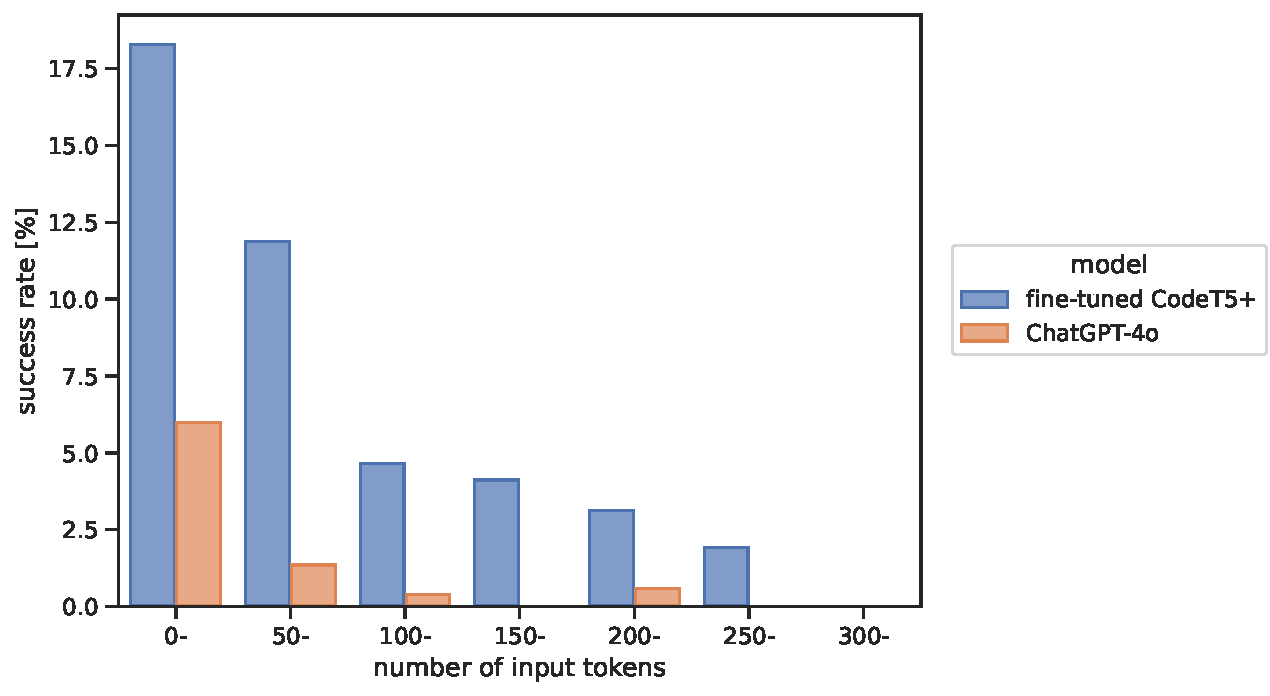
\includegraphics[width=1.0\linewidth]{Omori_fig/result.pdf}
\caption{result}
\label{fig-result}
\end{center}
\end{figure}


検証データセット5,962件のうち,CodeT5+をファインチューニングしたモデルでは598件,ChatGPT-4oでは117件が完全一致,特に入力プログラムのトークン数が50未満の場合には18.3\%が検証データセットにおいて変更先プログラムと完全に一致した.これは最新の対話型人工知能であるChatGPT-4oと比較しても約3倍高い成功率である.したがって,マイクロベンチマーク共有サービス上で比較されているプログラム(特に,実行の速い実装方法を用いたプログラム)は,広く普及したプログラムとは異なる実装方法が多く含まれていると示唆される.

以下にCodeT5+をファインチューニングしたモデルによる生成プログラムの実例を示す.

\begin{lstlisting}[caption=Result Success (Input), label=result-success-input,captionpos=t]
var VAR_1 = [];
for(var VAR_2 = 0; VAR_2 < 10; VAR_2++)
  VAR_1.push(VAR_2);
\end{lstlisting}

\begin{lstlisting}[caption=Result Success (Output), label=result-success-output,captionpos=t]
var VAR_1 = new Array(10);
for(var VAR_2 = 0; VAR_2 < 10; VAR_2++)
  VAR_1[VAR_2] = VAR_2;
\end{lstlisting}

\begin{lstlisting}[caption=Result Success (Generate), label=result-success-generate,captionpos=t]
var VAR_1 = new Array(10);
for(var VAR_2 = 0; VAR_2 < 10; VAR_2++)
  VAR_1[VAR_2] = VAR_2;
\end{lstlisting}

Listing~\ref{result-success-input},\ref{result-success-output},\ref{result-success-generate}は生成したプログラムが完全一致した実例である.
Listing~\ref{result-success-input}は検証データセットの1つの入力プログラム,Listing~\ref{result-success-output}はその期待される出力プログラム,Listing~\ref{result-success-generate}は実際にCodeT5+をファインチューニングしたモデルが生成したプログラムである.プログラム全体の完全一致によって成否を判定しているため,Listing~\ref{result-success-input}とListing~\ref{result-success-generate}は同一のプログラムである.Listing~\ref{result-success-input}およびListing~\ref{result-success-output}はいずれも長さ10の配列VAR\_1を宣言し,順に整数値で初期化するプログラムである.ただし,両者は配列の宣言方法が異なり,Listing~\ref{result-success-input}では空の配列初期化子,Listing~\ref{result-success-output}ではnew Array(10)を用いて初期化している.new Array(10)を用いる方が事前に配列の長さを確保しているため高速になると考えられる.また,宣言方法に応じて各プログラム3行目の初期化方法も異なる.Listing~\ref{result-success-generate}では正解プログラムと同様に,1行目の宣言方法と3行目の初期化方法の両方を修正できているため,提案モデルは複数行にわたる命令文を理解し,修正できることが分かる.

\begin{lstlisting}[caption=Result Failure (Input), label=result-failure-input,captionpos=t]
var VAR_1 = [];
for(var VAR_2 = 100000; VAR_2--; )
  VAR_1[VAR_2] = 0;
\end{lstlisting}

\begin{lstlisting}[caption=Result Failure (Output), label=result-failure-output,captionpos=t]
var VAR_1 = [];
for(var VAR_2 = 0; 100000 - VAR_2; VAR_2++; )
  VAR_1[VAR_2] = 0;
\end{lstlisting}

\begin{lstlisting}[caption=Result Failure (Generate), label=result-failure-generate,captionpos=t]
var VAR_1 = new Array(100000);
for(var VAR_2 = 100000; VAR_2--; )
  VAR_1[VAR_2] = 0;
\end{lstlisting}

Listing~\ref{result-failure-input},\ref{result-failure-output},\ref{result-failure-generate}は,生成したプログラムが完全一致はしていないが,意味的に等価なプログラムを生成した実例である.
Listing~\ref{result-failure-input}は検証データセットの1つの入力プログラム,Listing~\ref{result-failure-output}はその期待される出力プログラム,Listing~\ref{result-failure-generate}は実際にCodeT5+をファインチューニングしたモデルが生成したプログラムである.Listing~\ref{result-failure-input}とListing~\ref{result-failure-generate}は実装上は異なるプログラムであるが,目視で確認した結果,意味的に等価であり,このような生成プログラムに対して,次節で取り扱う.

また,Listing~\ref{result-failure-input}とListing~\ref{result-failure-output}はListing~\ref{result-success-input}およびListing~\ref{result-success-output}と同様に配列を初期化するプログラムである.CodeT5+をファインチューニングしたモデルはListing~\ref{result-success-generate}と同様に配列の宣言方法を空の配列初期化子からnew Array(100000)に修正したが,正解プログラムが別の箇所の修正を期待していたため,完全一致しなかった.このように,リファクタリングに失敗した事例の中には他の実装方法を学習したことによると考えられる失敗も確認できた.

このように,本結果は完全一致によってリファクタリング成否を判定したが,プログラムには多様な実装方法が存在するため,検証データセット内の正解プログラムと完全一致していない生成プログラムであっても,意味的に等価で入力プログラムよりも実行時間が短いことも考えられる.次節では,入力プログラムとの等価性を判定した上で実行時間を測定し,実行速度を改善した生成プログラムを特定する.もし,次節でもベースラインより実行が速くなったプログラムが多く存在すれば,本節の結果から,マイクロベンチマーク共有サービスにはリファクタリング性能の向上に有用な特有の実装方法が存在することが明らかになった.

\subsection{意味的な等価性に基づく判定結果}
プログラムには多様な実装方法が存在するため,検証データセット内の正解プログラムと完全一致していない生成プログラムであっても,意味的に等価で入力プログラムよりも実行時間が短いことも考えられる.そのため,\ref{subsec:clean}節で作成したアルゴリズムを用いて入力プログラムとの等価性を判定した上で,\ref{subsec:measureTime}節と同様の手法で実行時間を測定し,実行速度を改善した生成プログラムを特定する.

その結果,5,962件の検証データセットに対して,CodeT5+をファインチューニングしたモデルでは22件,ChatGPT-4oでは19件の生成プログラムが入力プログラムが,意味的に等価かつ入力プログラムよりも実行時間が短いことが分かった.
前節では,CodeT5+をファインチューニングしたモデルで598件,ChatGPT-4oで117件の生成プログラムが正解プログラムと完全に一致したため,本来,少なくともこれらのプログラムはすべて入力プログラムよりも実行時間が短いことが期待していた.しかし,前節でリファクタリング成功と判定されたほとんどの生成プログラムが入力プログラムと実行時間に有意な差が無いと判定された.これは,前処理の段階でプログラム中の使用されていない変数や関数を削除する等の改変を行った結果であると考えられる.

変数や関数の宣言・代入がインタプリタ言語にとって比較的に実行時間に影響の大きい処理であることは既に知られている\cite{Gong_2015}が,マイクロベンチマークのように非常に短いプログラムに対しては,特に大きく影響するという知見が得られた.

マイクロベンチマークはセットアッププログラムとテストプログラムに分かれており,テストプログラムによっては使用されていない変数や関数がセットアッププログラムで多く定義されていたことから,学習への悪影響を考慮して削除処理を行ったが,今後は事前に前処理を行った後に実行時間を測定することでモデルのより正確な修正性能を明らかにすることが望まれる.ただし,実行時間を測定する前に全通りの実装対に対して前処理を行うためには本研究の手順よりも長い処理時間を要することに留意する必要がある.

%あるいは,前処理の一部手順を適用しない,使用されていない変数や関数を残したプログラムを用いて検証することが考えられる.

%メモ:
%抽象化はするけど不要な変数は削除してないプログラムで検証すればよかったのでは? TODO

%%%%%%%%%%%%%%%%%%%%%
\section{妥当性への脅威}\label{sec:threats}
%%%%%%%%%%%%%%%%%%%%%

\subsection{内的妥当性}
本研究では,データセットの前処理に抽象構文木を使用している.その際,文章量の多いプログラムを抽象構文木に変換するために長時間かかるため,文字数が多い上位5\%のプログラムを除外し,95\%分位までのプログラムのみを対象とした.その結果,データセットはマイクロベンチマーク共有サービス上のプログラムを網羅できておらず,評価実験結果に影響を与える恐れがある.ただし,非常に長いプログラムの修正は現在の大規模言語モデルにとって困難なタスクであり,本研究でもCodeT5+の入出力最大長は512トークンに制限している.そのため,本研究の目的であるマイクロベンチマーク共有サービス上のプログラムを学習した大規模言語モデルの修正性能を明らかにする上での影響は小さいと考える.

本研究では,マイクロベンチマーク共有サービスJsPerfからプログラムを収集している.当該サービスは2020年にサービスを終了しているため,データセットには2020年7月までのプログラムしか含まれない.したがって,検証結果が現在でも高速な実装方法であるとは限らない.本研究では,収集データセットの中で,最新リビジョン(JsPerfには既存のマイクロベンチマークを修正し,新たなリビジョンとして保存する機能が有る)のプログラムセットのみをデータセットに使用することで,データセット内での古い実装方法の比重を抑えるように可能な限り努めた.より正確な結果を得るためには他のマイクロベンチマーク共有サービスから継続的にプログラムを収集する必要がある.

本研究ではJavaScriptを実行する際に,サーバサイドJavaScript動作環境であるNodeJSを使用している.NodeJSはJavaScriptエンジンとしてV8を採用しており,Google ChromeやMicrosoft EdgeをはじめとするChromiumベースのブラウザアプリケーションでも広く用いられている.一方で,SpiderMonkeyやJavaScriptCore等のJavaScriptエンジンを採用するJavaScript実行環境も存在する.JavaScriptエンジンが異なる環境ではJITコンパイルアルゴリズムも異なるため,本研究で作成した実装対が一般にV8以外のJavaScriptエンジンでも効果的なリファクタリングであるとは限らない.本研究の評価実験結果はV8エンジンに限定した結果であるが,方法論については他のJavaScriptエンジンについても同様の手順で進行できるものであると考える.

\subsection{外的妥当性}
本研究では,マイクロベンチマーク共有サービス上のプログラムを対象に深層学習モデルのリファクタリング性能を明らかにしたが,多くのマイクロベンチマークプログラムは非常に短く,演算結果の代入や出力が省略されていることが多い.また,効果的に実行速度の差を測定するために巨大な配列や長大なループが用いられている.そのため,ライブラリのように実用目的で十分に保守されたソフトウェアとはプログラムの実装方法やリファクタリング時の影響が異なると考えられる.

%%%%%%%%%%%%%%%%%%%%%%%%%%%
\section{おわりに}\label{sec:conc}
%%%%%%%%%%%%%%%%%%%%%%%%%%%
本研究では,マイクロベンチマーク共有サービスで公開される実行速度が向上するプログラムを収集し大規模なデータセットを作成し,このデータセットを用いて大規模言語学習モデルをファインチューニングすることで実行を高速化するプログラムに自動リファクタリングするモデルを作成した.本研究で提案するモデルと,既存の対話型人工知能ChatGPT-4oの修正性能を比較した結果,マイクロベンチマーク共有サービス上のプログラムに対しては,正解プログラムとの完全一致に基づいてChatGPT-4oより約3倍も多くリファクタリングに成功した.評価実験の結果から,マイクロベンチマーク共有サービス上で比較されているプログラム(特に,実行の速い実装方法を用いたプログラム)には,広く普及したプログラムとは異なる実装方法が多く含まれていることが示唆される.一方で,実際の高速化効果に関しては実験手順に不備があり,十分に調査することができなかった.

本研究では,実行高速化のためのリファクタリング自動化に向けて,より高速な実装方法が存在することが明らかなマイクロベンチマークデータセット内で評価実験を行った.今後はGitHub上で開発されているOSS等を対象にした,実用目的のプログラムに対する修正性能を明らかにすることを目指す.

%\begin{acknowledgment}
%\end{acknowledgment}


\begin{thebibliography}{10}

\bibitem{Falleri_2014}
    J.R. Falleri, F. Morandat, X. Blanc, M. Martinez, and M. Monperrus,
    "Fine-grained and accurate source code differencing,"
    in Proceedings of the 29th ACM/IEEE International Conference on Automated Software Engineering (ASE),
    2014,
    pp.313-324.
\bibitem{Gong_2015}
    L. Gong, M. Pradel, and K. Sen,
    "JITProf: pinpointing JIT-unfriendly JavaScript code,"
    in Proceedings of the 2015 10th Joint Meeting on Foundations of Software Engineering (ESEC/FSE),
    2015,
    pp.357-368.
\bibitem{Selakovic_2016}
    M. Selakovic, and M. Pradel,
    "Performance issues and optimizations in JavaScript: an empirical study,"
    in Proceedings of the 38th International Conference on Software Engineering (ICSE),
    2016,
    pp.61-72.
\bibitem{Selakovic_2017}
    M. Selakovic, T. Glaser, and M. Pradel,
    "An actionable performance profiler for optimizing the order of evaluations,"
    in Proceedings of the 26th ACM SIGSOFT International Symposium on Software Testing and Analysis (ISSTA),
    2017,
    pp.170-180.
\bibitem{Saiki_2021}
    K. Saiki, and A. Ihara,
    "Linkage of Similar Code Snippets Assessed in the Micro Benchmark Service jsPerf,"
    in Proceedings of the 21th IEEE International Working Conference on Source Code Analysis and Manipulation (SCAM),
    2021,
    pp.247-251.
\bibitem{Shirafuji_2023}
    A. Shirafuji, Y. Oda, J, Suzuki, M. Morishita, and Y. Watanobe,
    "Refactoring Programs Using Large Language Models with Few-shot Examples,"
    in Proceedings of the 30th Asia-Pacific Software Engineering Conference (APSEC),
    2023,
    pp.151-160.
\bibitem{Wang_2023}
    Y. Wang, H. Le, A. D. Gotmare, N. D. Q. Bui, J. Li, and S. C. H. Hoi,
    "CodeT5+: Open Code Large Language Models for Code Understanding and Generation,"
    arXiv preprint,
    2023.
\bibitem{Ishizue_2024}
    R. Ishizue, K. Sakamoto, H. Washizaki, and Y. Fukazawa,
    "Improved Program Repair Methods using Refactoring with GPT Models,"
    in Proceedings of the 55th ACM Technical Symposium on Computer Science Education (SIGCSE),
    2024,
    pp.569-575.

\end{thebibliography}

\end{document}
